
\mychapter{함수의 극한}{}

\section{$x \to \infty$, $x \to -\infty$의 의미}
어떤 실수 $x$가 한없이 커지는 것을 $x \to \infty$라 표기하고, 한없이 작아지는 것을 $x \to -\infty$라 표기합니다.

\section{좌극한, 우극한, 극한}
\subsection{좌극한 $\lim_{x \to a-}$}
\begin{center}
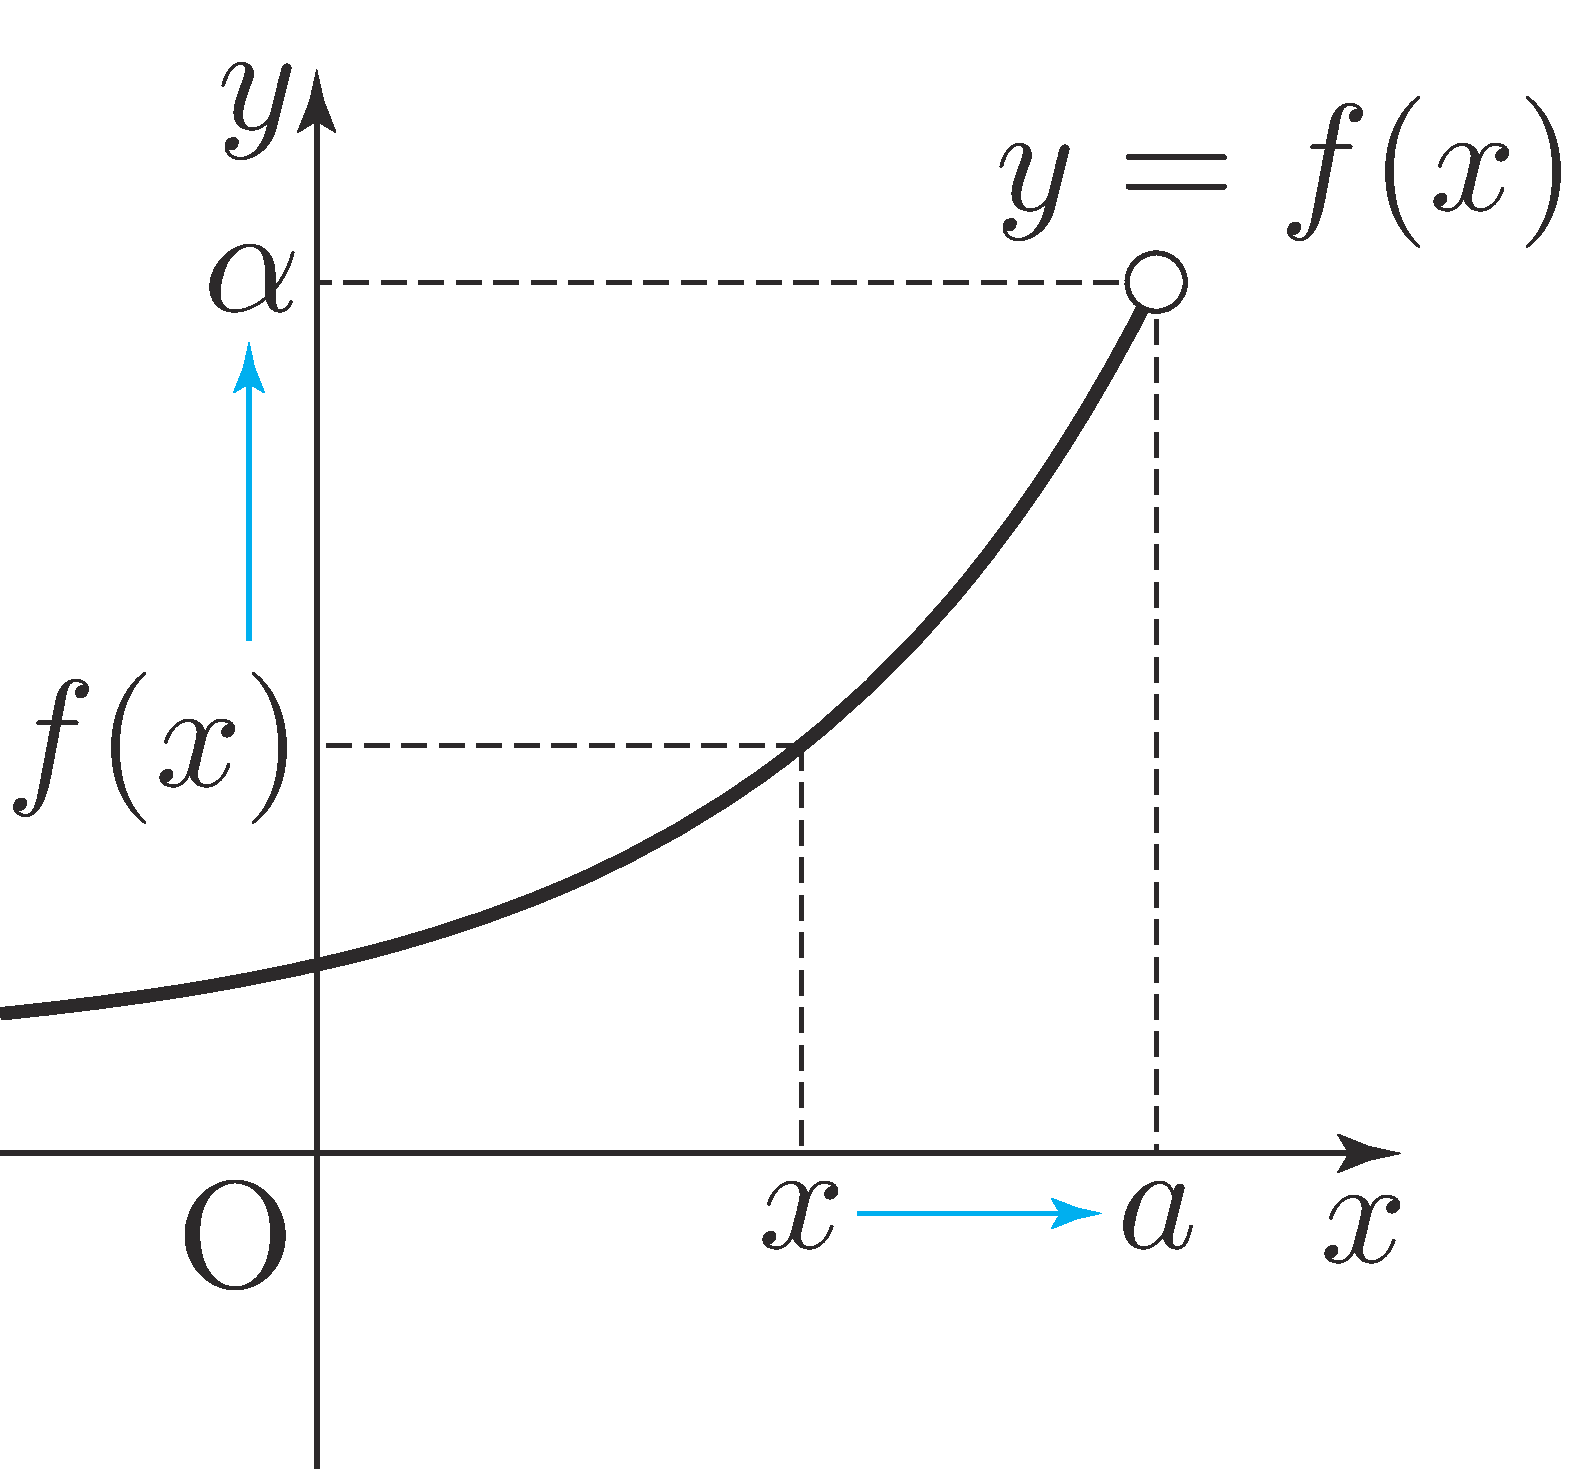
\includegraphics[scale=\pgfkeysvalueof{picsize}]{DBs/pic/zerr_02.pdf}\
\end{center}일반적으로 함수 $f\left( x \right) $에서 $x$의 값이 $a$보다 작은 값을 가지면서 $a$에 한없이 가까워질 때, $f\left( x \right) $의 값이 $\alpha$에 한없이 가까워지면 $\alpha$를 $x=a$에서 함수 $f\left( x \right) $의 \term{좌극한}{}이라 하고, $\lim_{x \to a-}f\left( x \right) = \alpha$라 표기합니다.
\subsection{우극한 $\lim_{x \to a+}$}
\begin{center} 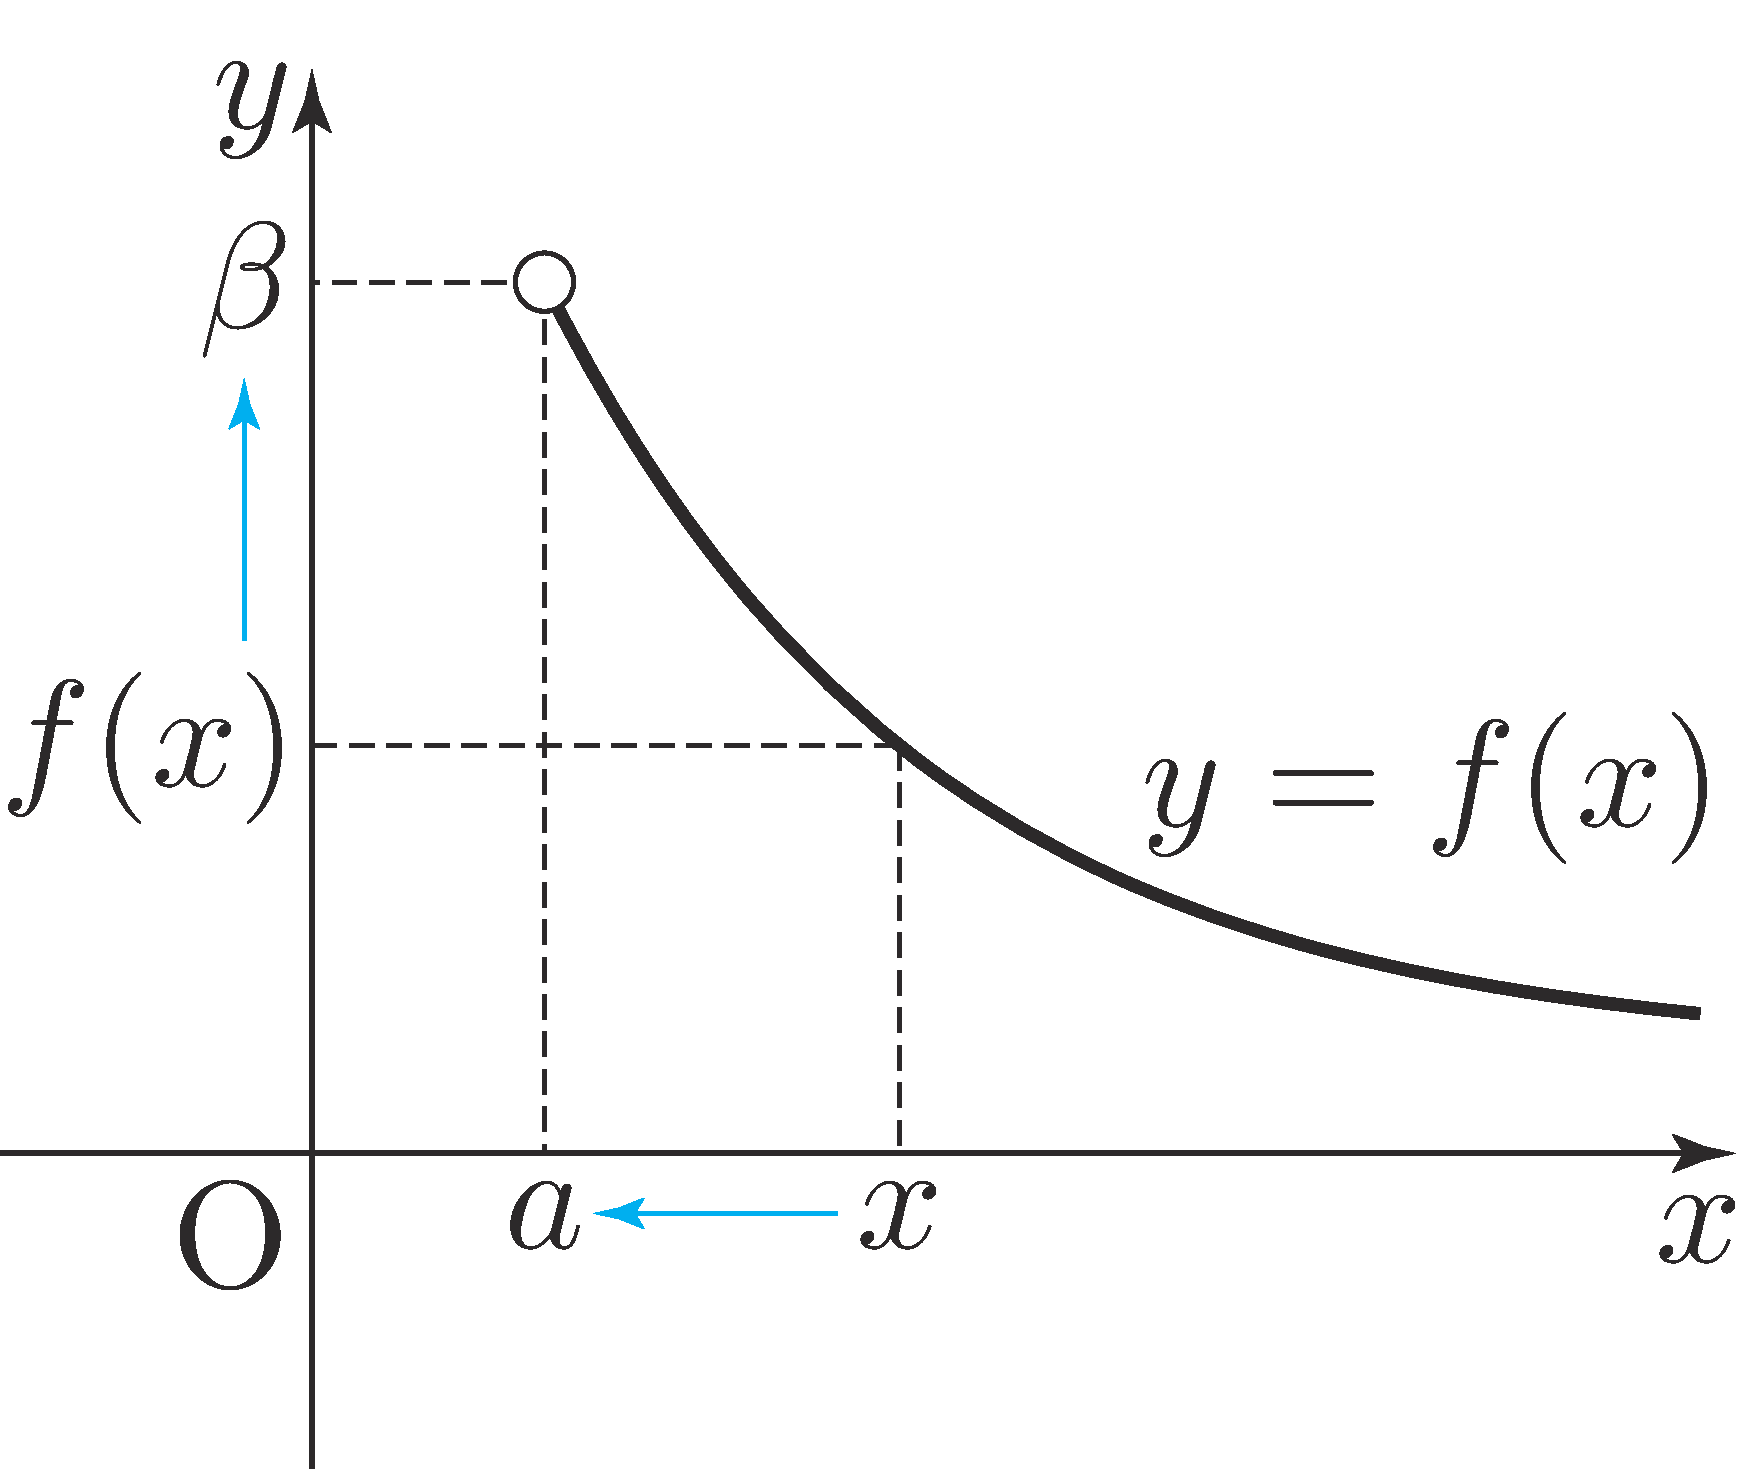
\includegraphics[scale=\pgfkeysvalueof{picsize}]{DBs/pic/zerr_03.pdf}\
	\end{center}일반적으로 함수 $f\left( x \right) $에서 $x$의 값이 $a$보다 큰 값을 가지면서 $a$에 한없이 가까워질 때, $f\left( x \right) $의 값이 $\beta$에 한없이 가까워지면 $\beta$를 $x=a$에서 함수 $f\left( x \right) $의 \term{우극한}{}이라 하고, $\lim_{x \to a+}f\left( x \right) = \beta$라 표기합니다.
\clearpage
\subsection{함수의 수렴과 극한 $\lim_{x \to a}$}
\begin{center} 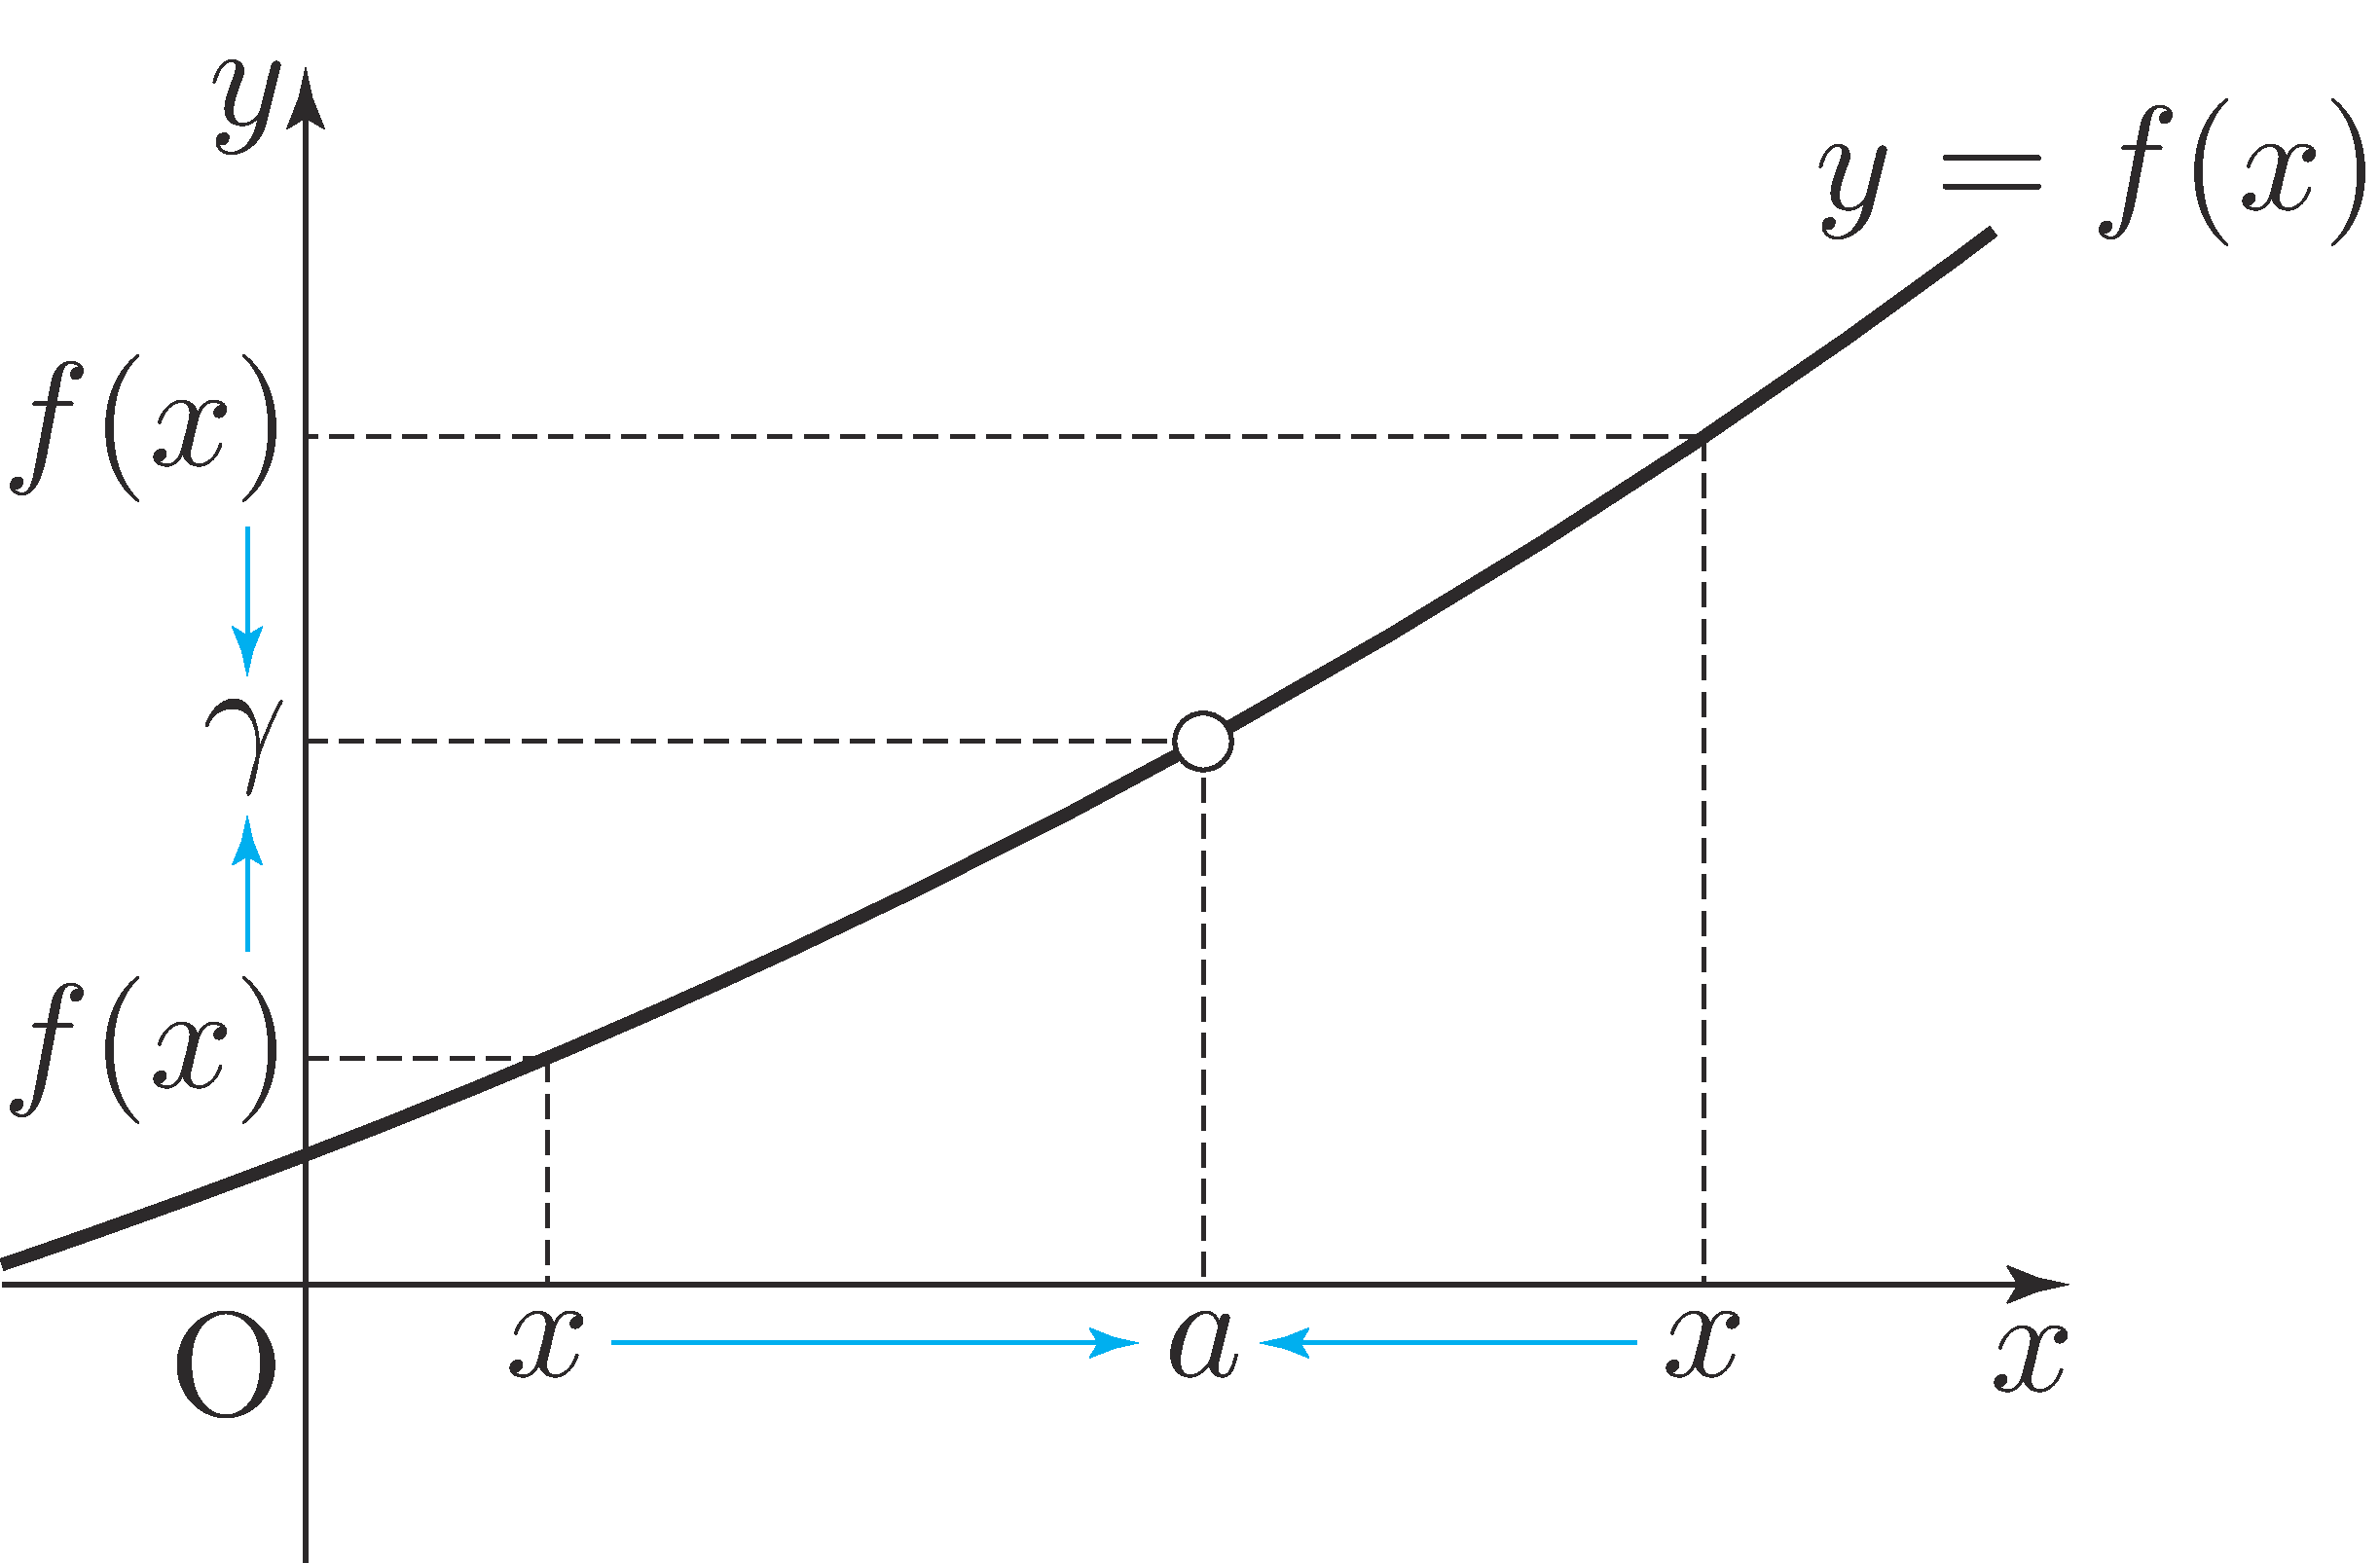
\includegraphics[scale=\pgfkeysvalueof{picsize}]{DBs/pic/zerr_04.pdf}\
	\end{center}함수 $f\left( x \right) $가 $x=a$에서 좌극한과 우극한이 각각 존재하고 두 값이 $\gamma$로 서로 같다면, $x$의 값이 $a$와 다른 값을 가지면서 $a$에 한없이 가까워질 때, $f\left( x \right) $의 값이 $\gamma$에 한없이 가까워집니다. 이때 함수 $f\left( x \right) $는 $\gamma$에 \term[함수의 극한]{수렴}{2}한다고 합니다. 한편 $\gamma$를 $x=a$에서 함수 $f\left( x \right) $의 \term[함수의 극한]{극한값}{2} 또는 \term[함수의 극한]{극한}{2}이라 하고, $\lim_{x \to a}f\left( x \right) =\gamma$라 표기합니다.

함수의 극한이 존재하면 좌극한과 우극한이 각각 존재하고 그 값은 서로 같습니다.

\subsection{함수의 발산과 극한 $\lim_{x \to a}$}

\begin{figure}[h]
	\centering \subfloat[][$f(x) \to \infty$인 경우]{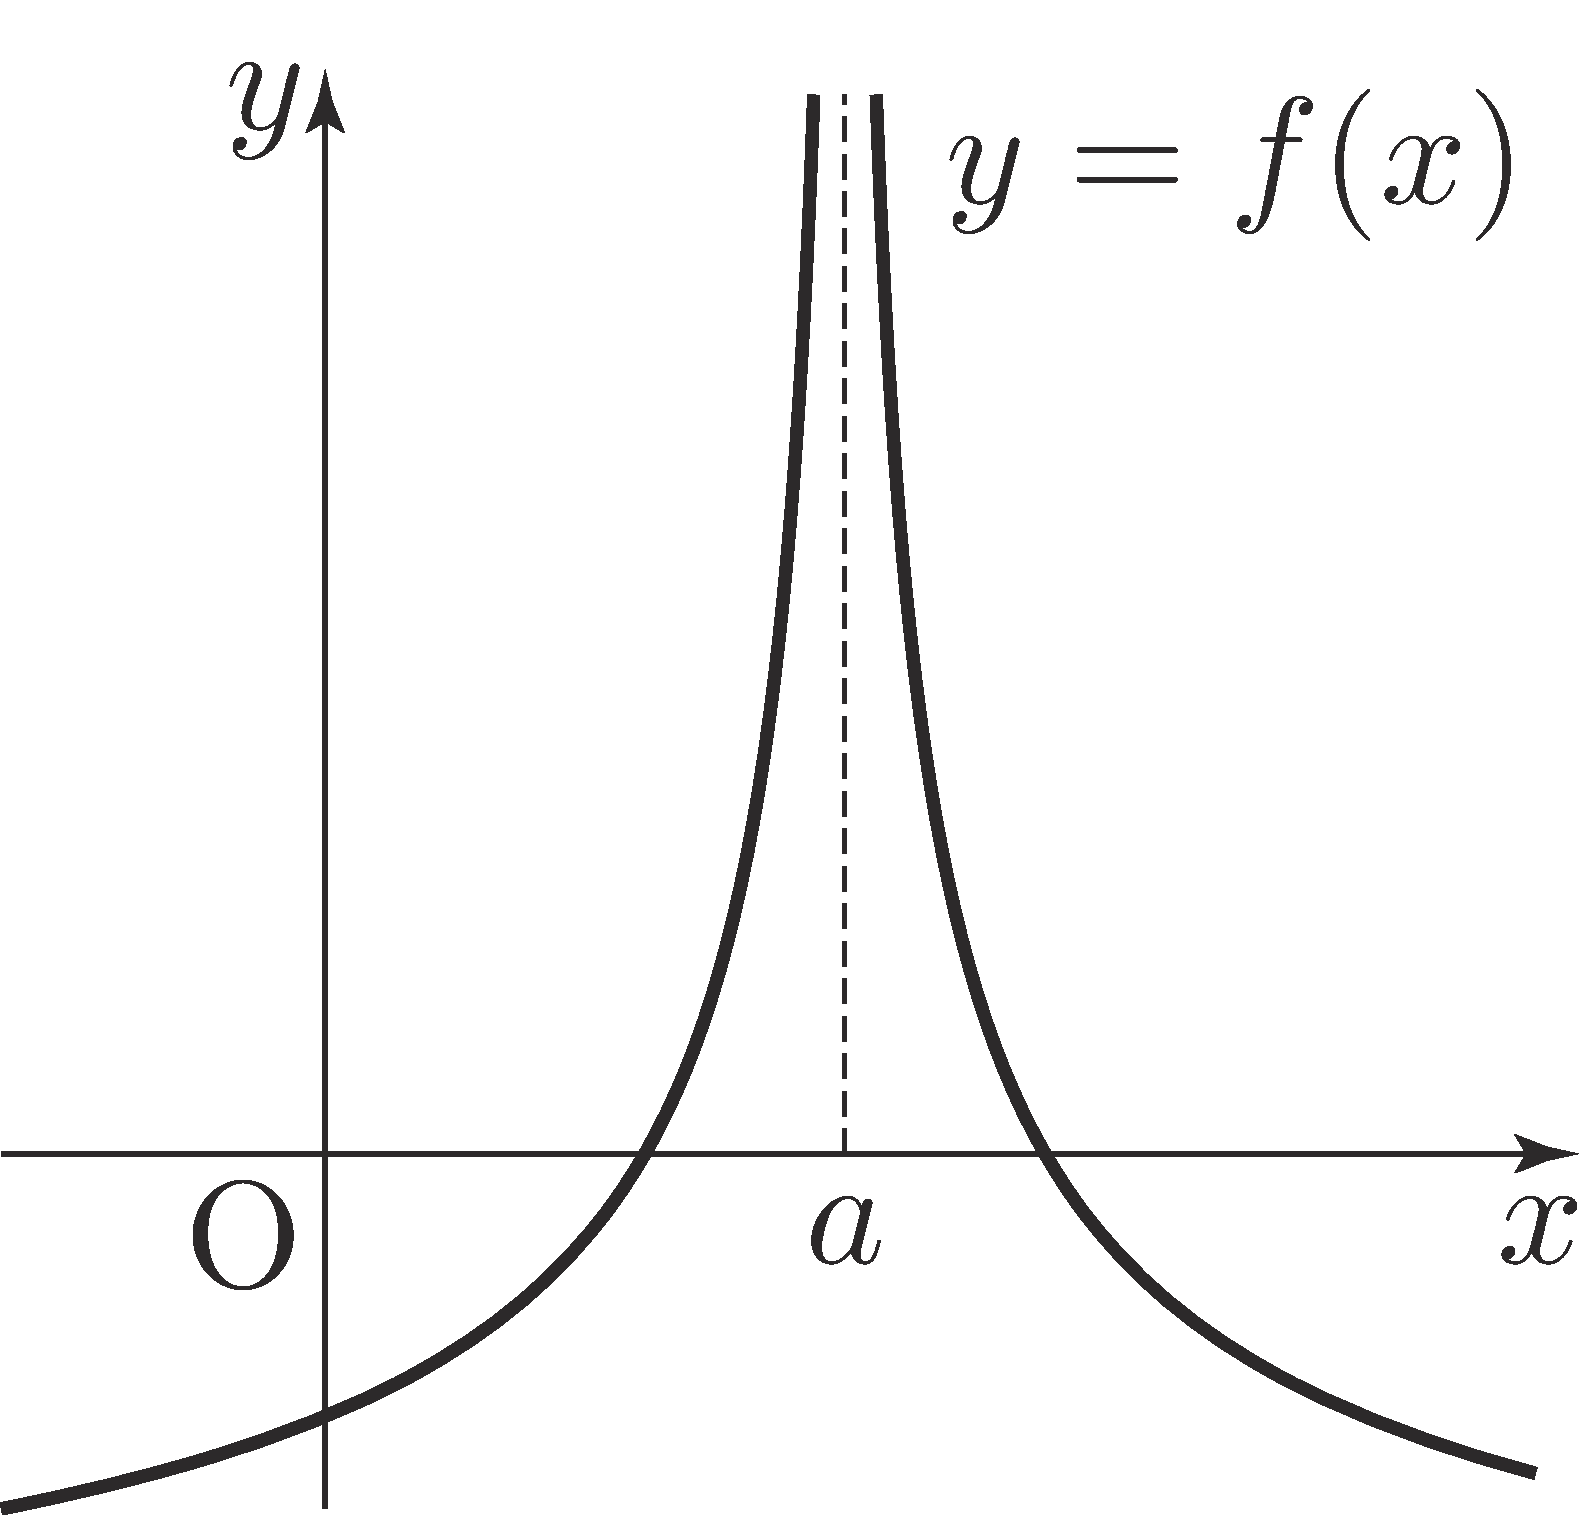
\includegraphics[scale=\pgfkeysvalueof{picsize}]{DBs/pic/zerr_05_1.pdf}}\
	\qquad\qquad
	\centering \subfloat[][$f(x) \to -\infty$인 경우]{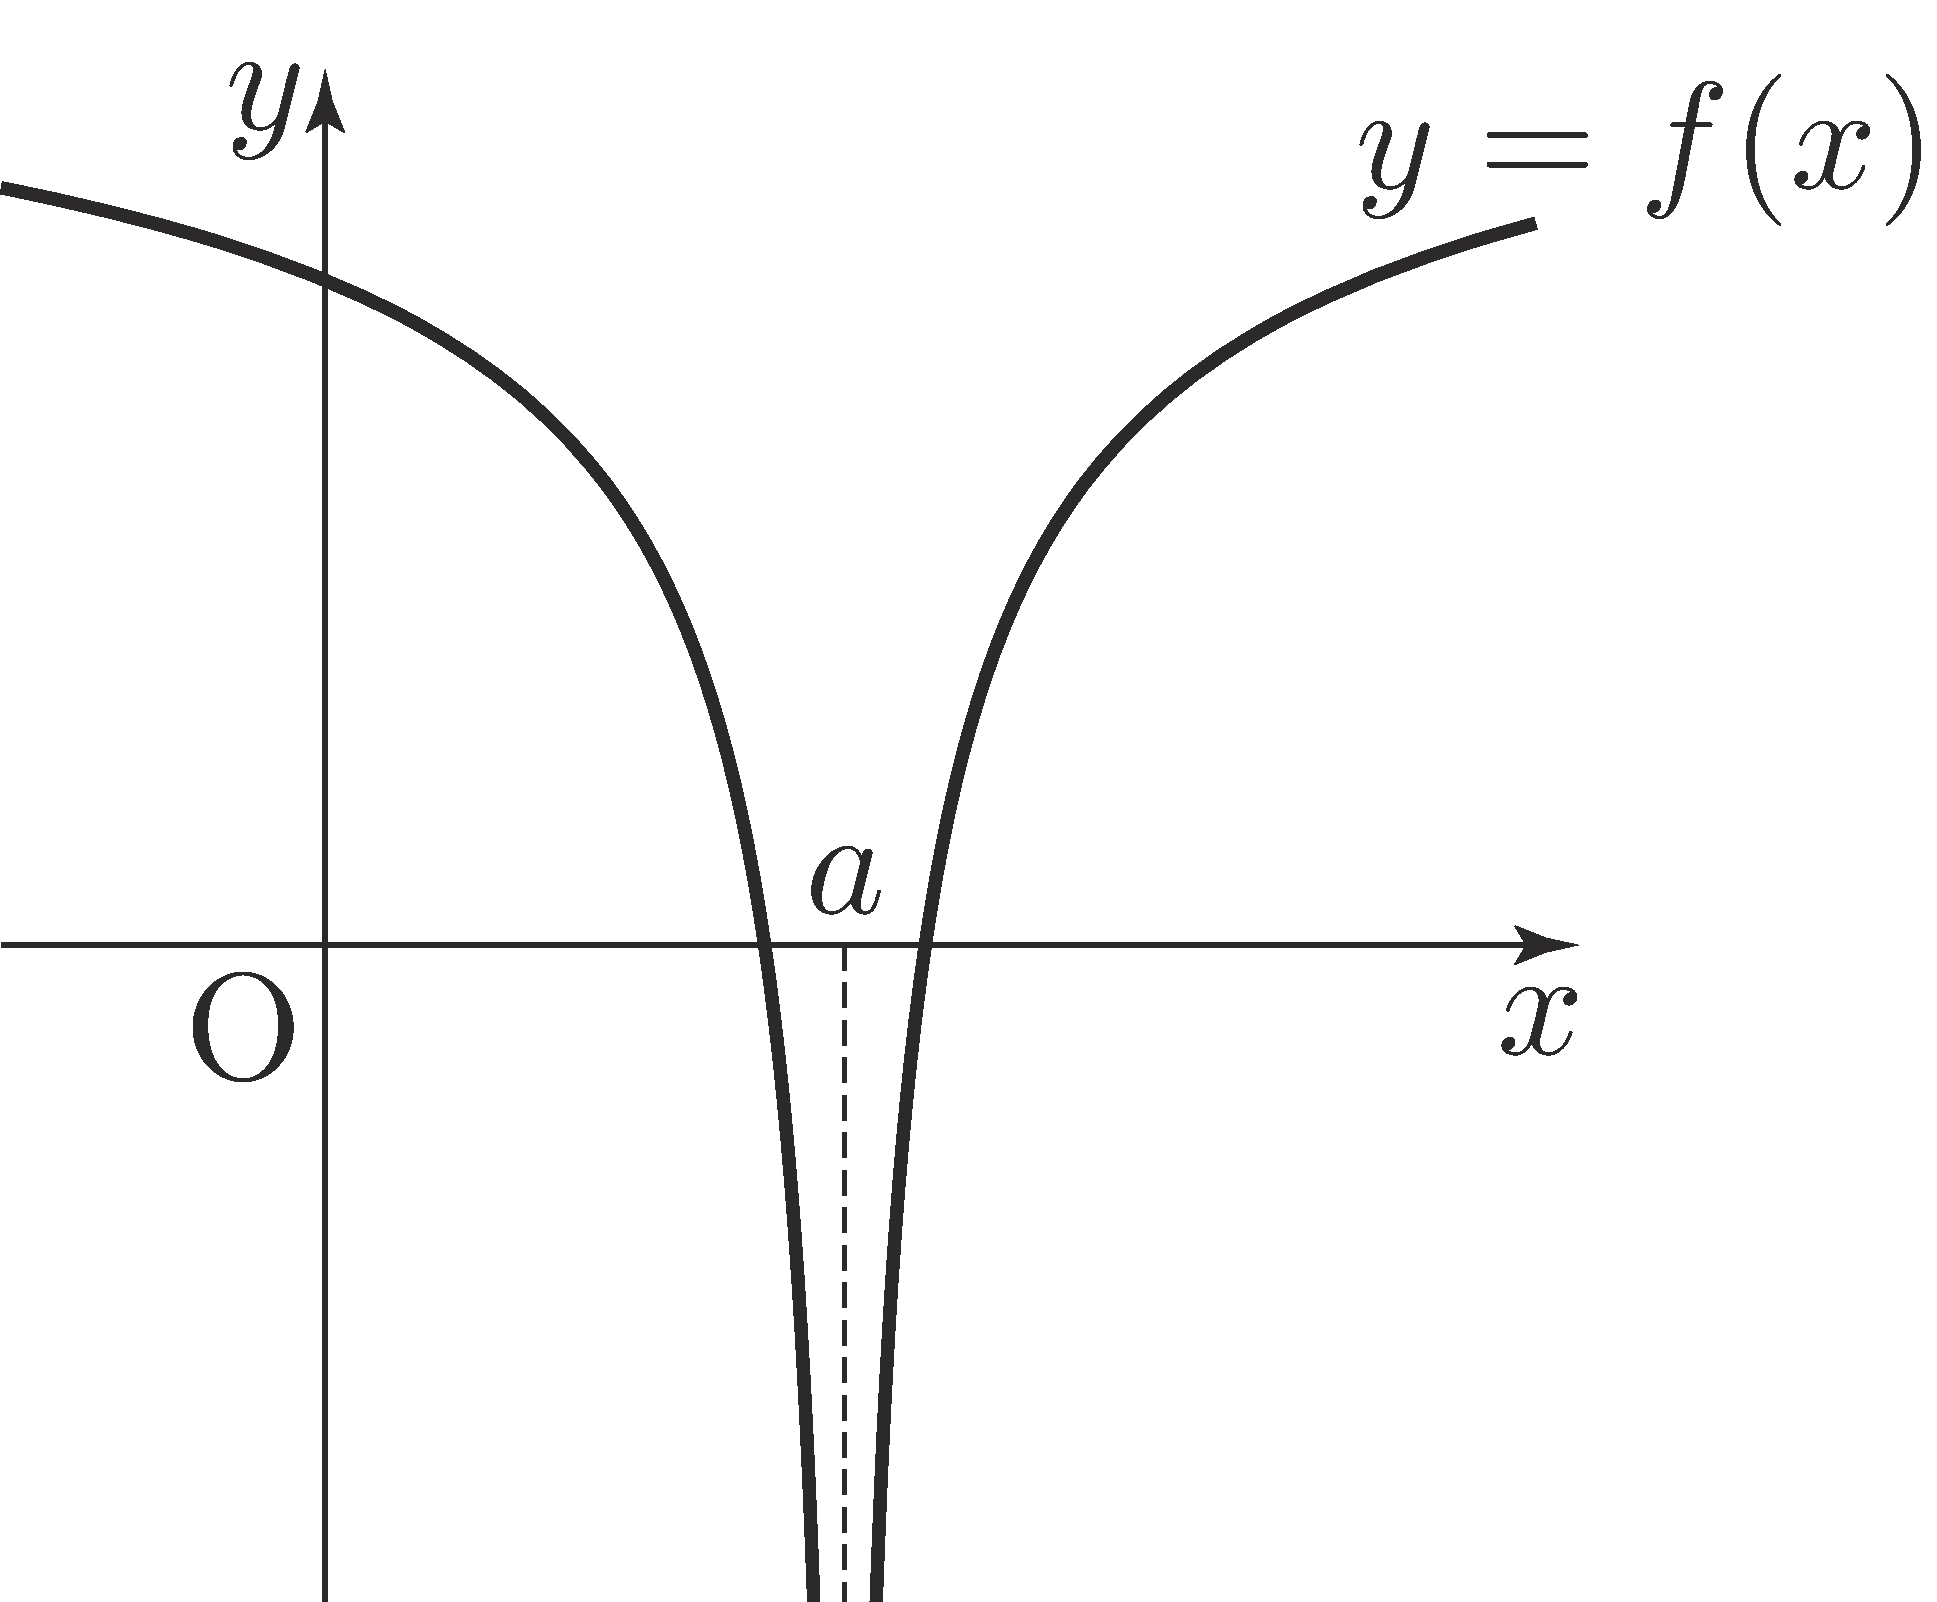
\includegraphics[scale=\pgfkeysvalueof{picsize}]{DBs/pic/zerr_05_2.pdf}}\
	\end{figure}
$x \to a-$일 때 $f\left( x \right) \to \infty$이고 $x \to a+$일 때 $f\left( x \right) \to \infty$이면 `$x=a$에서 함수 $f\left( x \right) $는 \term[함수의 극한]{양의 무한대로 발산}{2}한다'고 하며, $\lim_{x \to a} f\left( x \right) = \infty$라 표기합니다.\mn{이 표현은 등식이 아님에 주의합시다.}{} 

$x \to a-$일 때 $f\left( x \right) \to -\infty$이고 $x \to a+$일 때 $f\left( x \right) \to -\infty$이면 `$x=a$에서 함수 $f\left( x \right) $는 \term[함수의 극한]{음의 무한대로 발산}{2}한다'고 하며, $\lim_{x \to a} f\left( x \right) = -\infty$라 표기합니다.\mn{이 표현은 등식이 아님에 주의합시다.}{} 

교과서에서는 지금까지의 내용 외에는 $x=a$에서의 함수의 발산을 명시적으로 정의하지는 않았지만, 다음의 세 가지를 자연스럽게 정의할 수 있습니다.
\begin{enumerate}[label=\onum*]
    \item $x=a$에서 좌극한이 존재하지 않으면 $x=a$에서 함수는 발산합니다.
    \item $x=a$에서 우극한이 존재하지 않으면 $x=a$에서 함수는 발산합니다.
    \item $x=a$에서 좌극한과 우극한이 각각 존재하지만 서로 같지 않으면 $x=a$에서 함수는 발산합니다. 
\end{enumerate}



\subsection{$\lim_{x \to \infty}$, $\lim_{x \to -\infty}$}
일반적으로 함수 $f\left( x \right) $에서 $x$의 값이 한없이 커질 때, $f\left( x \right) $의 값이 일정한 값 $\alpha$에 한없이 가까워지면 $\lim_{x \to \infty}f\left( x \right) =\alpha$라 표기합니다.

일반적으로 함수 $f\left( x \right) $에서 $x$의 값이 음수이면서 그 절댓값이 한없이 커질 때, $f\left( x \right) $의 값이 일정한 값 $\beta$에 한없이 가까워지면 $\lim_{x \to -\infty}f\left( x \right) =\beta$라 표기합니다.

지금까지 배운 내용을 바탕으로 $x \to \infty$ 또는 $x \to -\infty$일 때 양의 무한대 또는 음의 무한대로 발산하는 상황에 대한 표기를 자연스럽게 정의할 수 있습니다.\mn{네 표기 모두 등식이 아님을 주의합시다.}{}
\begin{alignat*}{2}
\lim_{x \to \infty}f\left( x \right) &= \infty\quad \lim_{x \to \infty}f\left( x \right) &&= -\infty\\
\lim_{x \to -\infty}f\left( x \right) &= \infty\quad \lim_{x \to -\infty}f\left( x \right) &&= -\infty\\
\end{alignat*}
\begin{remark}{왜 네 표기 모두 등식이 아닌가요?}%{}
    우리는 교육과정에서 실수(가끔 복소수까지)에 대한 등식만을 다룹니다. 그런데 $\infty$는 실수가 아니므로, 주어진 식은 등식이 아닙니다. 이러한 표현은 그저 등식의 표현 방법만 빌렸을 뿐임을 주의합시다.
    
    다만 발산하는 함수에서와 달리, 수렴하는 함수에 대하여 극한값을 등호를 이용하여 표현할 때에는 좌변과 우변이 모두 실수이므로 등식이 맞습니다.
\end{remark} 
\subsection{수렴하는 함수의 극한에 대한 기본 성질}\term[함수의 극한]{수렴하는 함수의 극한에 대한 기본 성질}{0}
수렴하는 두 함수 $f \left( x \right) $, $g\left( x \right)  $에 대하여 $\lim f\left( x \right)  = \alpha$, $\lim g\left( x \right) = \beta$일 때, 다음이 성립합니다.\mn{$\lim{}$의 아랫첨자가 서로 같을 때에만 이용할 수 있습니다. 예를 들어 $\lim_{x \to a}f\left( x \right) = \alpha$, $\lim_{x \to \infty} g\left( x \right) =\beta$일 때에는 이 성질을 이용할 수 없습니다.}{}
\begin{thmbox}
    \begin{enumerate}[label=\onum*]
        \item $\lim \left\{ f\left( x \right) + g\left( x \right)   \right\}  = \lim f\left( x \right) + \lim g\left( x \right)  = \alpha + \beta$
        \item $\lim \left\{ f\left( x \right) - g\left( x \right)   \right\} = \lim f\left( x \right)  - \lim g\left( x \right) = \alpha - \beta$
        \item $\lim \left\{ k f\left( x \right)  \right\} = k\lim f\left( x \right)  = k\alpha$\quad(단, $k$는 상수)
        \item $\lim f\left( x \right)g\left( x \right)    =  \left\{ \lim f\left( x \right) \right\}   \times \left\{ \lim g\left( x \right) \right\}  = \alpha \beta$
        \item $\lim\dfrac{f\left( x \right) }{g\left( x \right) }= \dfrac{\displaystyle\lim f\left( x \right) }{\displaystyle\lim g\left( x \right) } = \dfrac{\alpha}{\beta}$\quad(단, $\beta \ne 0$)
    \end{enumerate}
\end{thmbox}





\clearpage
\subsection{함수의 극한의 대소관계}\term[함수의 극한]{대소관계}{0}
일반적으로 함수의 극한에 대하여 $x\to a$인 극한에 대하여 다음과 같은 대소관계가 성립합니다.
\begin{thmbox}
    $\lim_{x \to a} f\left( x \right) =\alpha$, $\lim_{x \to a} g\left( x \right) = \beta$ ($\alpha$, $\beta$는 실수)일 때, $a$를 포함하는 어떤 열린구간에 포함된 $x$ 중 $a$가 아닌 모든 실수 $x$에 대하여
   \begin{enumerate}[label={\onum*}]
       \item $f\left( x \right) \le g\left( x \right) $이면 $\alpha \le \beta$이다.
       \item $f\left( x \right) \le h\left( x \right) \le g\left( x \right) $이고 $\alpha=\beta$이면 $\lim_{x \to a}h\left( x \right) =\alpha$이다.
   \end{enumerate}
\end{thmbox}

$x\to \infty$인 극한\mn{$x\to -\infty$일 때에도 마찬가지로 성립합니다.}{}에 대해서도 다음과 같은 대소관계가 성립합니다.
\begin{thmbox}
    $\lim_{x \to \infty} f\left( x \right) =\alpha$, $\lim_{x \to \infty} g\left( x \right) = \beta$ ($\alpha$, $\beta$는 실수)일 때,
   \begin{enumerate}[label={\onum*}]
       \item $f\left( x \right) \le g\left( x \right) $이면 $\alpha \le \beta$이다.
       \item $f\left( x \right) \le h\left( x \right) \le g\left( x \right) $이고 $\alpha=\beta$이면 $\lim_{x \to \infty}h\left( x \right) =\alpha$이다.
   \end{enumerate}
\end{thmbox}
각 경우는 다음을 내포하고 있습니다.\begin{center}
    $f\left( x \right) < g\left( x \right) $이면 $\alpha \le \beta$이다\\
    $f\left( x \right) < h\left( x \right) < g\left( x \right) $이고 $\alpha=\beta$이면 $\lim_{x \to \infty}h\left( x \right) =\alpha$이다
\end{center}따라서 \textbf{\color{cyan}부등식에 극한을 취할 땐 원래 부등식에 등호가 없더라도 극한을 취한 후에는 등호를 붙인다}라고 생각하면 됩니다.


\clearpage

\section{함수의 연속}
\subsection{한 점에서의 연속의 정의}
함수 $f\left( x \right) $가 다음을 만족시킬 때,  함수 $f\left( x \right) $가 $x=a$에서 \term{연속}{}이라고 합니다.\mn{사실 ③은 ①과 ②를 내포하고 있습니다. ③의 식은 등식이고, 우변에 $f\left( a \right) $라 쓰려면 $f\left( a \right) $가 존재해야 하므로 ①이 전제되어 있습니다. 또한 $f\left( a \right) $는 실수이므로, 좌변도 실수입니다. 즉 $\lim_{x \to a}f\left( x \right) $가 존재하고 \mbox{그 값이} $f\left( a \right) $라는 의미이므로 ①이 전제되어 있습니다.}{}
\begin{justbox}
\begin{enumerate}[label={\onum*}]
    \item $x=a$에서 정의되어 있다. (함숫값 $f\left( a \right) $가 존재한다)
    \item $\lim_{x \to a}f\left( x \right) $가 존재한다.
    \item $\lim_{x \to a}f\left( x \right) = f\left( a \right) $이다.
\end{enumerate}
\end{justbox}

\subsection{연속함수(정의역 전체에서의 연속)의 정의}
다음을 만족시키는 함수 $f(x)$를 \term{연속함수}{}라 합니다.
\begin{justbox}
정의역 내의 모든 실수 $k$에 대하여 함수 $f\left( x \right) $가 $x=k$에서 연속이다.
\end{justbox}
다음을 만족시키는 함수 $f(x)$를 `구간 $\OOI{a}{b}$에서 연속' 또는 `구간 $\OOI{a}{b}$에서 연속함수'라 합니다.
\begin{justbox}
$a<k<b$인 모든 실수 $k$에 대하여 $\lim_{x \to k} f\left( x \right) = f\left( k \right) $이다.
\end{justbox}
다음을 만족시키는 함수 $f(x)$를 `구간 $\CCI{a}{b}$에서 연속' 또는 `구간 $\CCI{a}{b}$에서 연속함수'라 합니다.\mn{$\coi{a}{b}$, $\oci{a}{b}$, $\coi{a}{\infty}$, $\oci{-\infty}{b}$와 같이 구간의 한 쪽 끝만 닫힌 경우에도 동일한 원칙을 적용합니다. 열린 구간 끝에서는 추가적인 연속성을 판정하지 않고, 닫힌 구간 끝에서만 연속성을 따져주면 됩니다.}{}
\begin{justbox}
\begin{enumerate}[label={\onum*}]
    \item  구간 $\OOI{a}{b}$에서 연속이다.
    \item $\lim_{x \to a+} f(x)= f\left( a \right) $
    \item $\lim_{x \to b-} f(x)= f\left( b \right) $    
\end{enumerate}
\end{justbox}
한편 실수 전체의 집합에서 연속인 함수를 `$\OOI{-\infty}{\infty}$에서 연속함수'라고 하며, 반열린(반닫힌) 구간에서의 연속은 위의 정의에 따라 자연스럽게 정의할 수 있을 것입니다.
\clearpage
\subsection{연속함수의 성질}\term{연속함수의 성질}{0}
$x=a$에서 연속인 두 함수 $f\left( x \right) $, $g\left( x \right) $와 상수 $c$에 대하여, 다음 함수도 $x=a$에서 연속입니다.\mn{`연속의 정의'와 `수렴하는 함수의 극한의 성질'을 이용하여 증명할 수 있습니다.}{}
\begin{selection}{label={\onum* }}
    \item $cf\left( x \right) $
    \item $f\left( x \right) + g\left( x \right)  $
    \item $f\left( x \right) - g\left( x \right) $
    \item $f\left( x \right)g\left( x \right)  $
    \item $\dfrac{f\left( x \right)}{g\left( x \right)} $  (단, $g\left( a \right)  = 0$일 때에는 $x=a$에서 연속이 아님)
\end{selection}

\subsection{다항함수와 유리함수의 연속성}
`연속함수의 성질'과 `상수함수 $y=a$와 일차함수 $y=x$가 실수 전체의 집합에서 연속'\mn{이에 대해서는 증명 없이 받아들입니다.}{}임을 이용하면 다항함수가 실수 전체의 집합에서 연속임을 보일 수 있습니다.

\term{다항함수}{}란 함수식이 다항식인, 즉 함수식이 다음과 같은 꼴인 함수를 말합니다.
\begin{align*} f\left( x \right) = a_n x^n + a_{n-1}x^{n-1} + \cdots + a_1 x + a_0 = \sum_{k=0}^{n}a_k x^k\end{align*}
다항함수는 `상수함수와 일차함수의 곱'으로 이루어진 항들의 합으로 이루어져 있으므로, 연속함수의 성질에 의해 연속함수입니다.\mn{수학적귀납법을 이용하여 증명할 수 있습니다.}{}

유리함수는 두 다항함수 $f\left( x \right) $, $g\left( x \right) $에 대하여 $\dfrac{g\left( x \right) }{f\left( x \right) }$로 나타내어지는 함수입니다. 따라서 연속함수의 성질에 의하여 분모 $f\left( x \right) $의 값이 $0$이 되도록 하는 $x$의 값을 제외한 모든 실수에서 연속입니다.
\clearpage
\subsection{\Mmi{} 정리}
\begin{center}
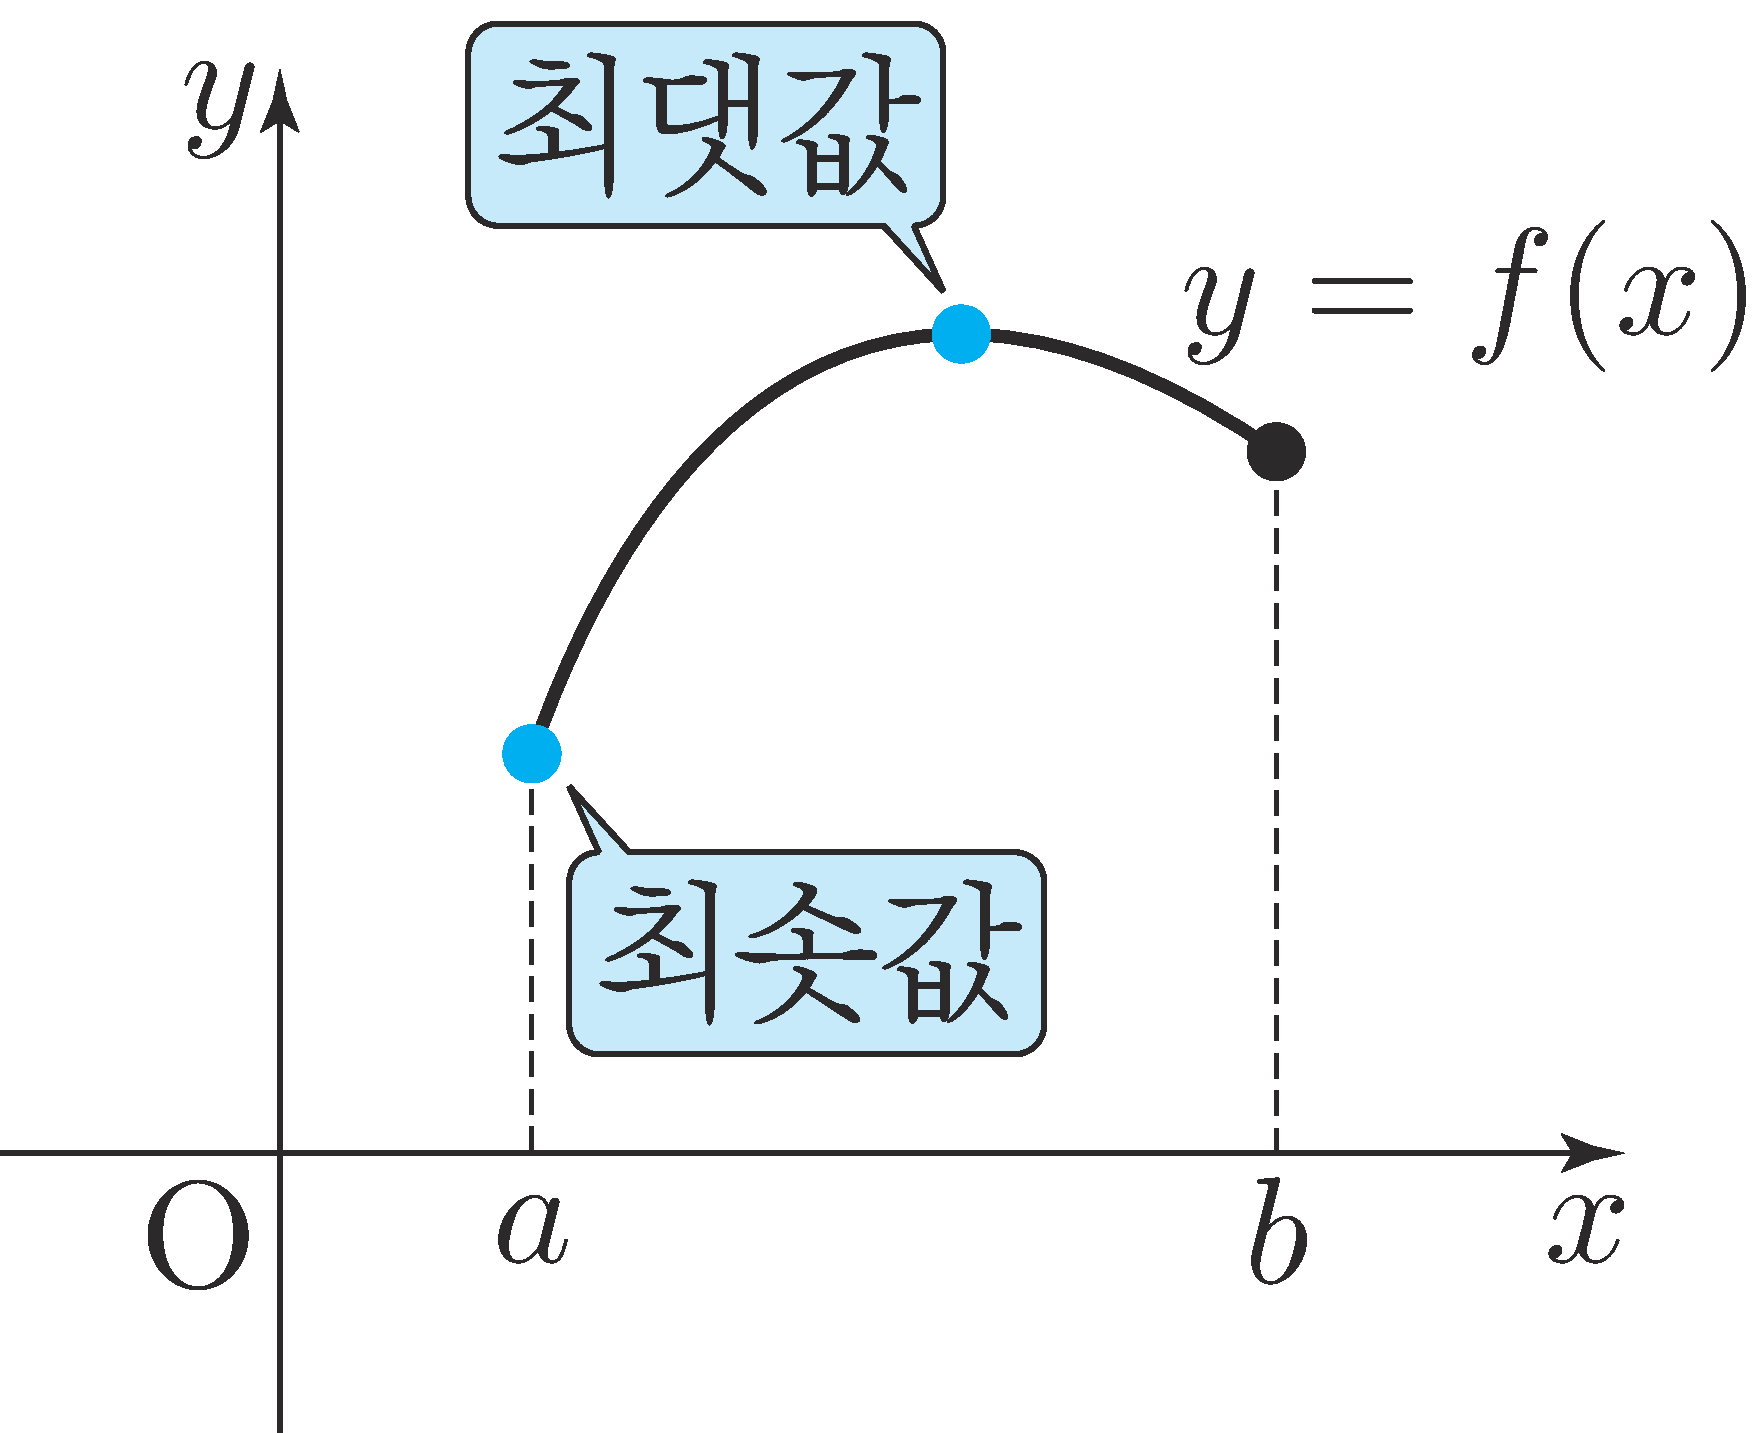
\includegraphics[scale=\pgfkeysvalueof{picsize}]{DBs/pic/zerg_04.pdf}\
\end{center}\term[최대최소 정리]{\Mmi{} 정리}{3}는 증명 없이 받아들이는 연속함수에 대한 정리입니다.
\begin{thmbox}
    함수 $f\left( x \right) $가 닫힌구간 $\CCI ab$에서 연속이면 함수 $f\left( x \right) $는 이 구간에서 반드시 최댓값과 최솟값을 갖는다. 
\end{thmbox}
\clearpage\begin{center} 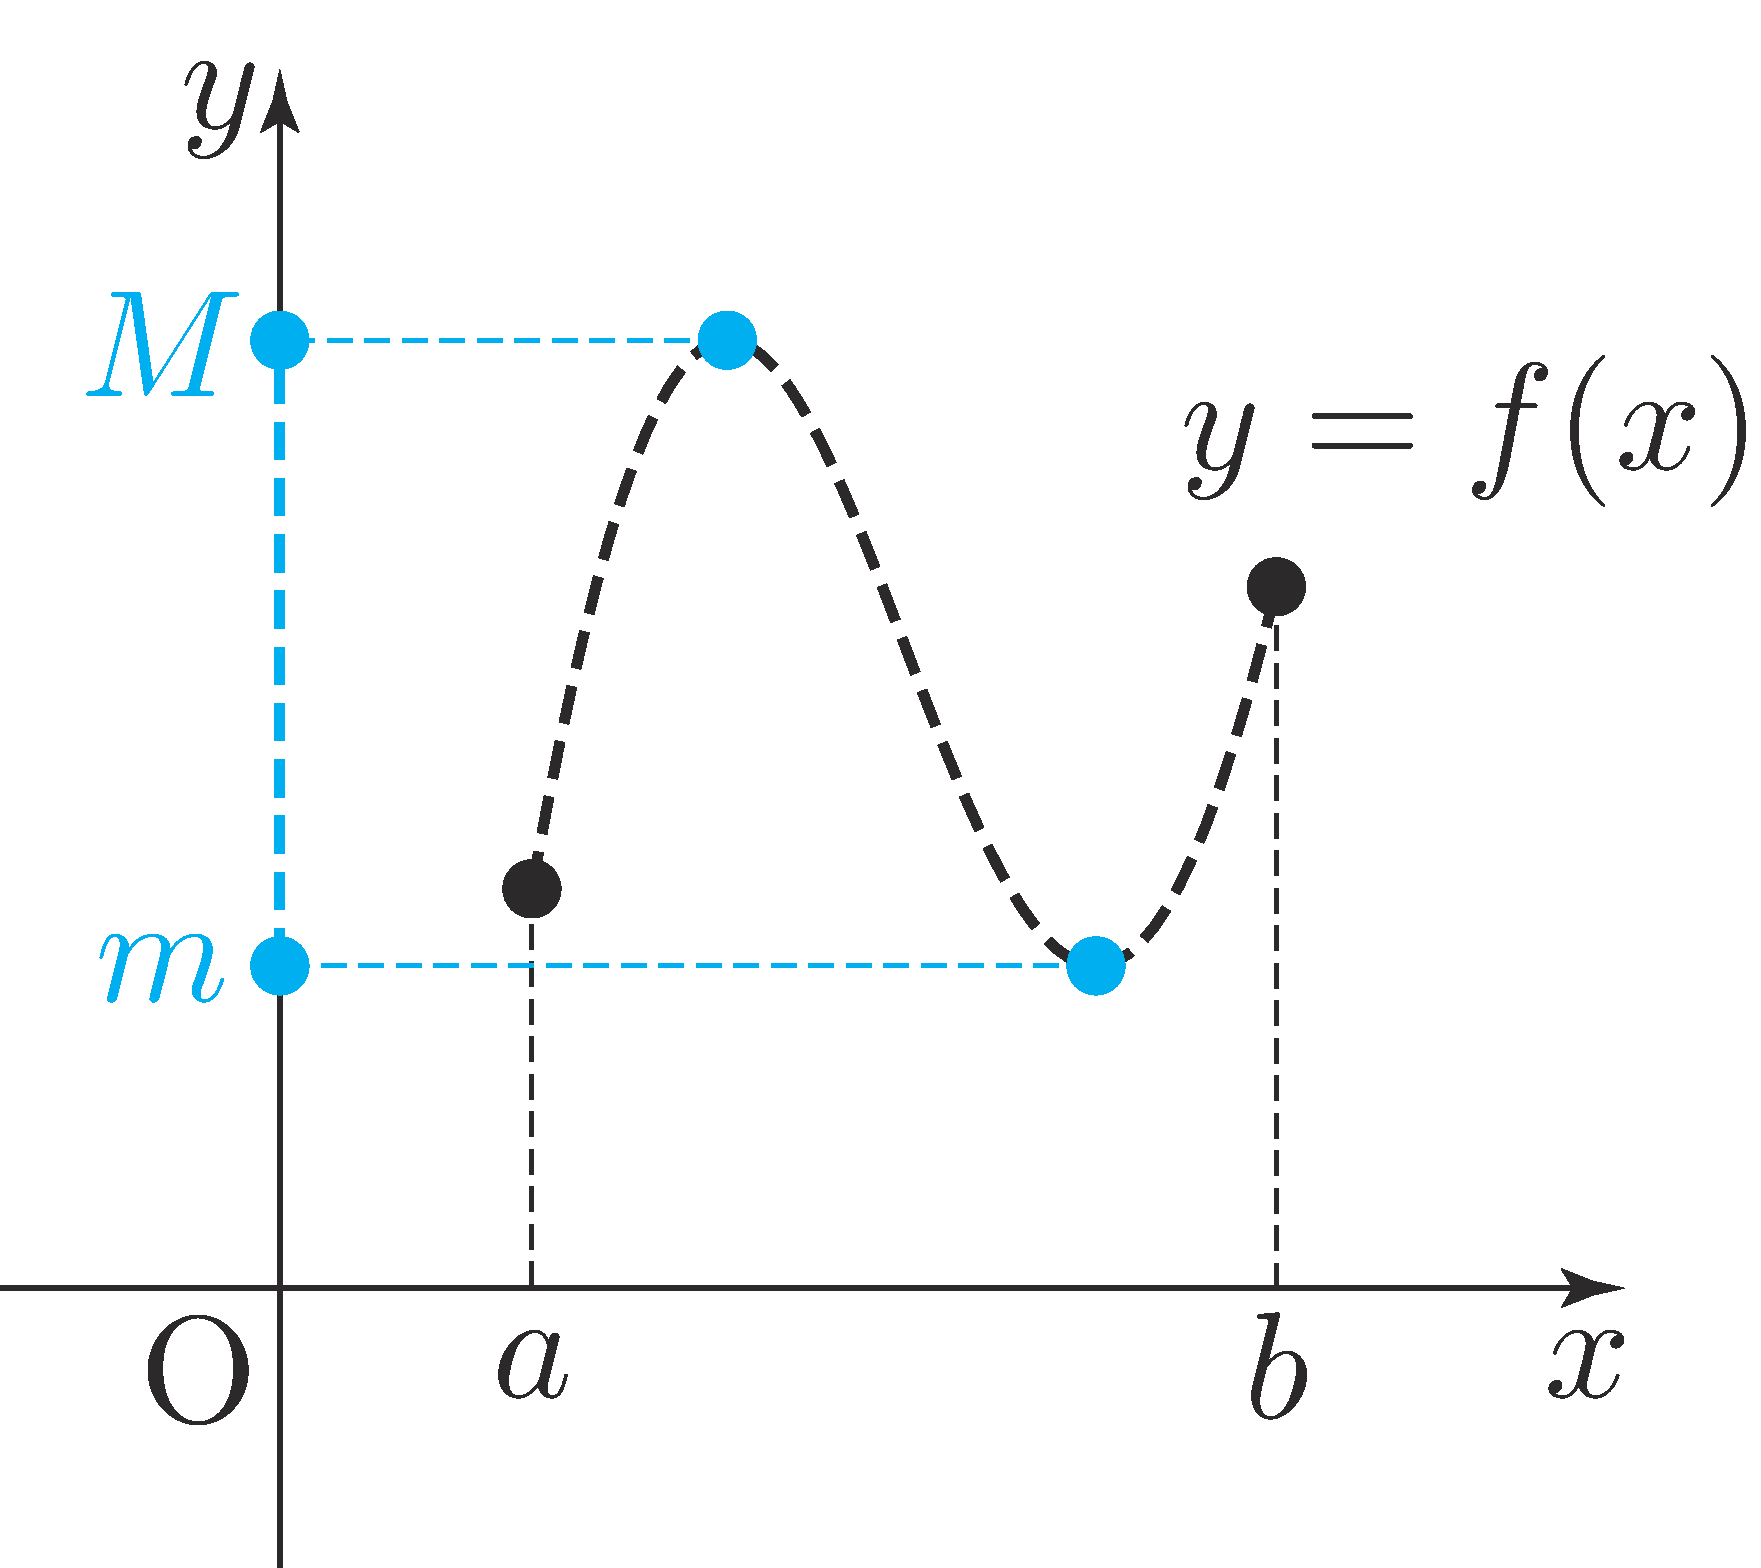
\includegraphics[scale=\pgfkeysvalueof{picsize}]{DBs/pic/zerg_05.pdf}\
	\end{center}\Mmi{} 정리에 따르면, 함수 $f\left( x \right) $의 닫힌구간 $\CCI ab$에서의 최댓값과 최솟값을 각각 $M$, $m$이라 할 때, $f\left( x \right) $의 치역의 원소 $y$에 대하여 $m \le y \le M$이 항상 성립합니다.\mn{단 \Mmi{} 정리만으로는 $y$가 $m$과 $M$ 사이의 모든 값을 \dotemph{빠짐없이} 가질 수 있음을 이야기하는 것은 아닙니다. 그저 어떤 \mbox{$y$값을} 가져오더라도 \mbox{$m$보다는} 크거나 같고, \mbox{$M$보다는} 작거나 같다는 의미입니다. \dotemph{빠짐없이 갖는다는 의미}는 바로 다음 페이지에서 다룹니다.}{}

\subsection{사잇값 정리}
\begin{center} 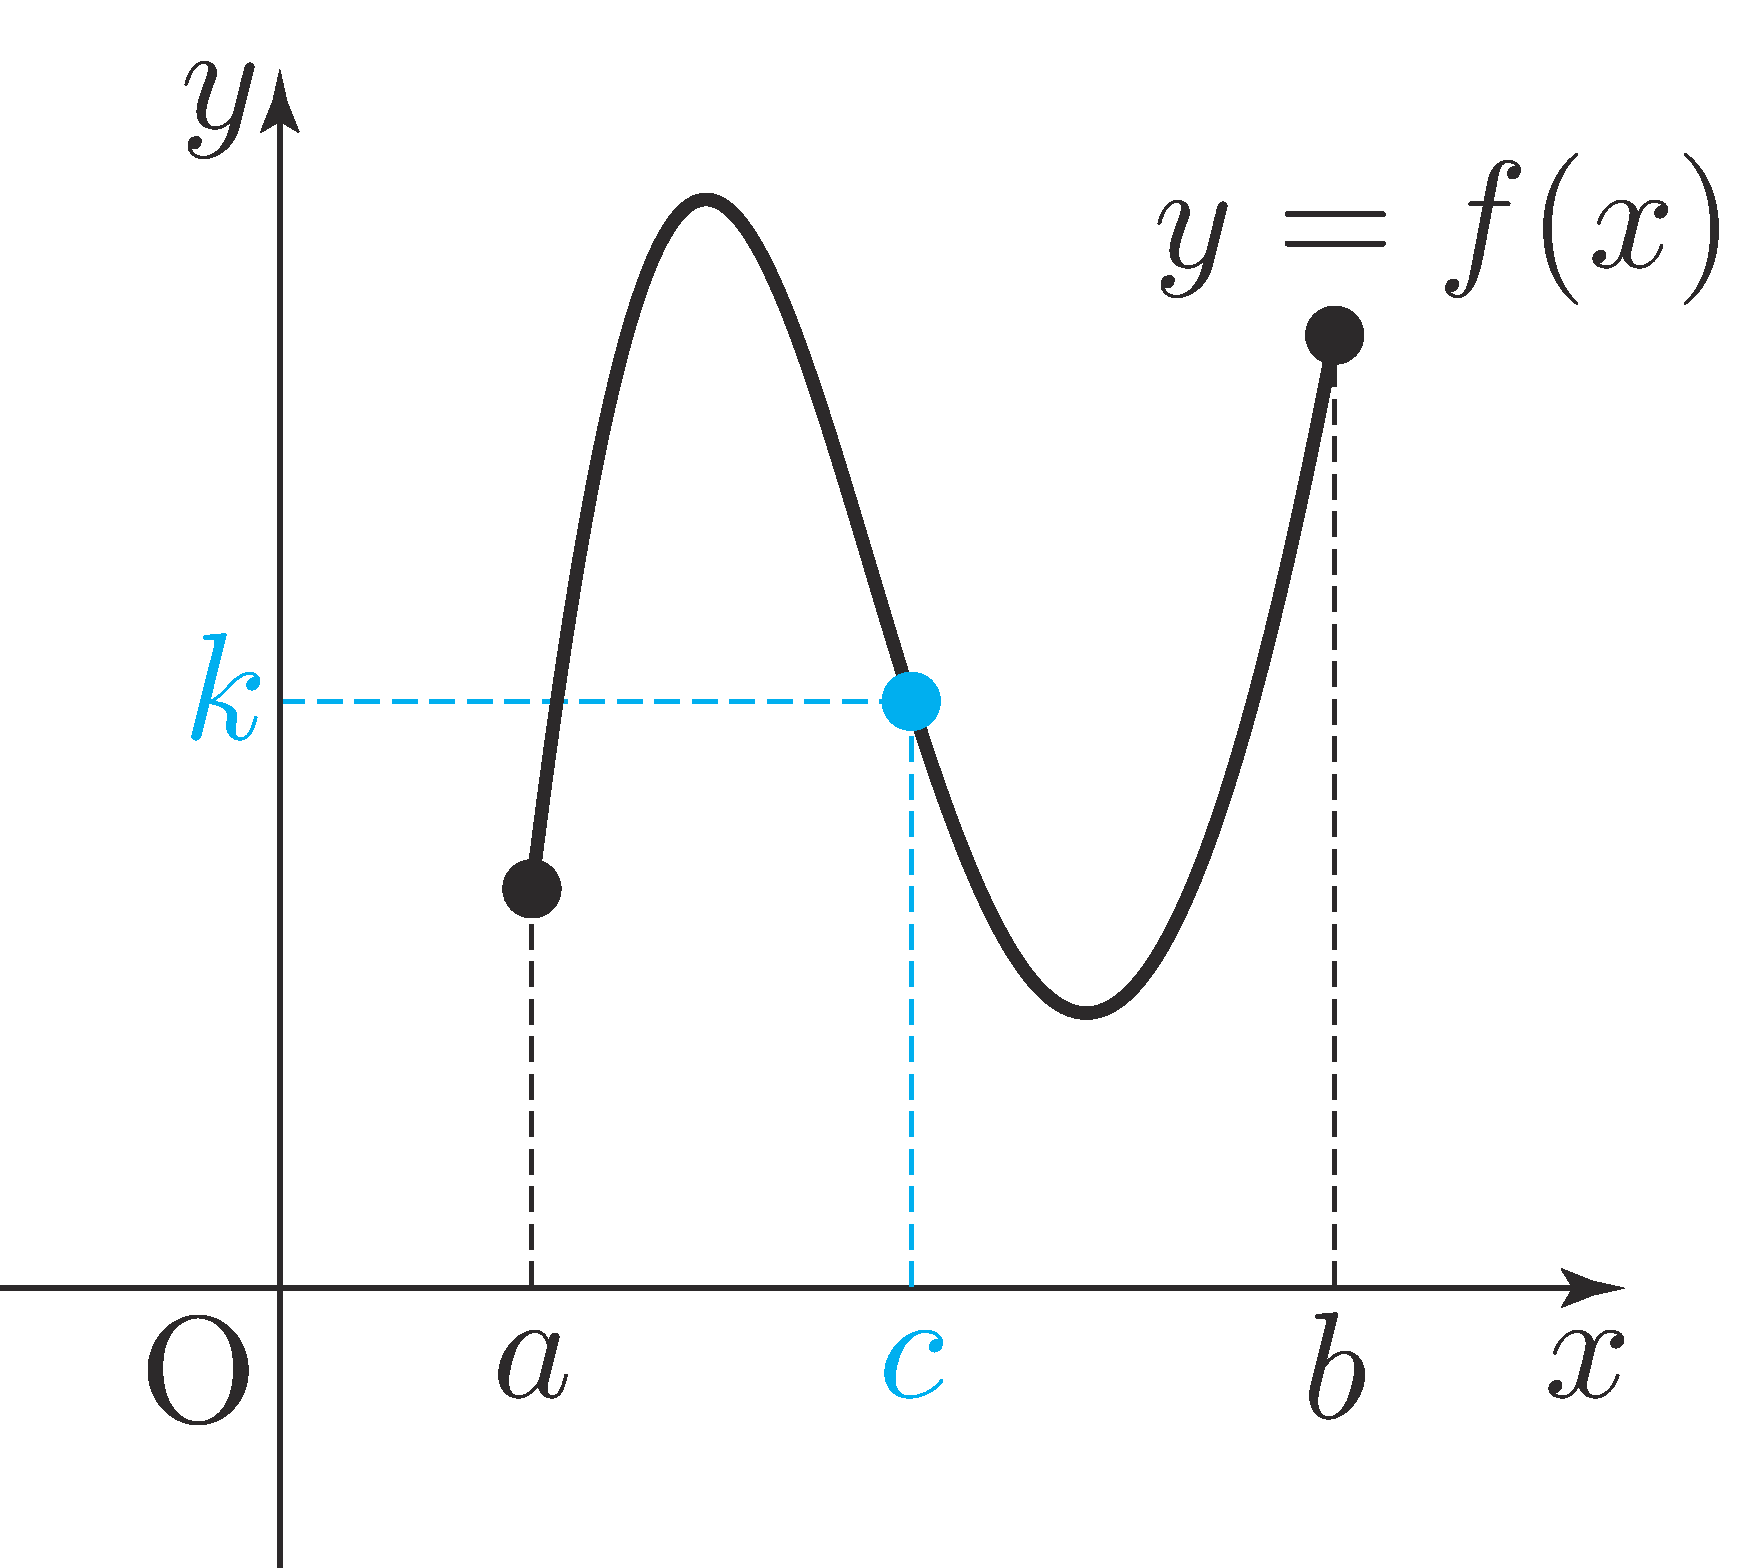
\includegraphics[scale=\pgfkeysvalueof{picsize}]{DBs/pic/zerg_06.pdf}\
	\end{center}\term{사잇값 정리}{}는 증명 없이 받아들이는 연속함수에 대한 정리입니다.
\begin{thmbox}
    함수 $f\left( x \right) $가 닫힌구간 $\CCI{a}{b}$에서 연속이고 $f\left( a \right) \ne f\left( b \right) $이면, $f\left( a \right) $보다는 크고 $f\left( b \right) $보다는 작은 임의의 실수 $k$에 대하여
    \begin{center}
        $a<c<b$, $f\left( c \right) =k$
    \end{center}    를 만족시키는 실수 $c$가 적어도 하나 존재한다.
\end{thmbox}
\begin{center} 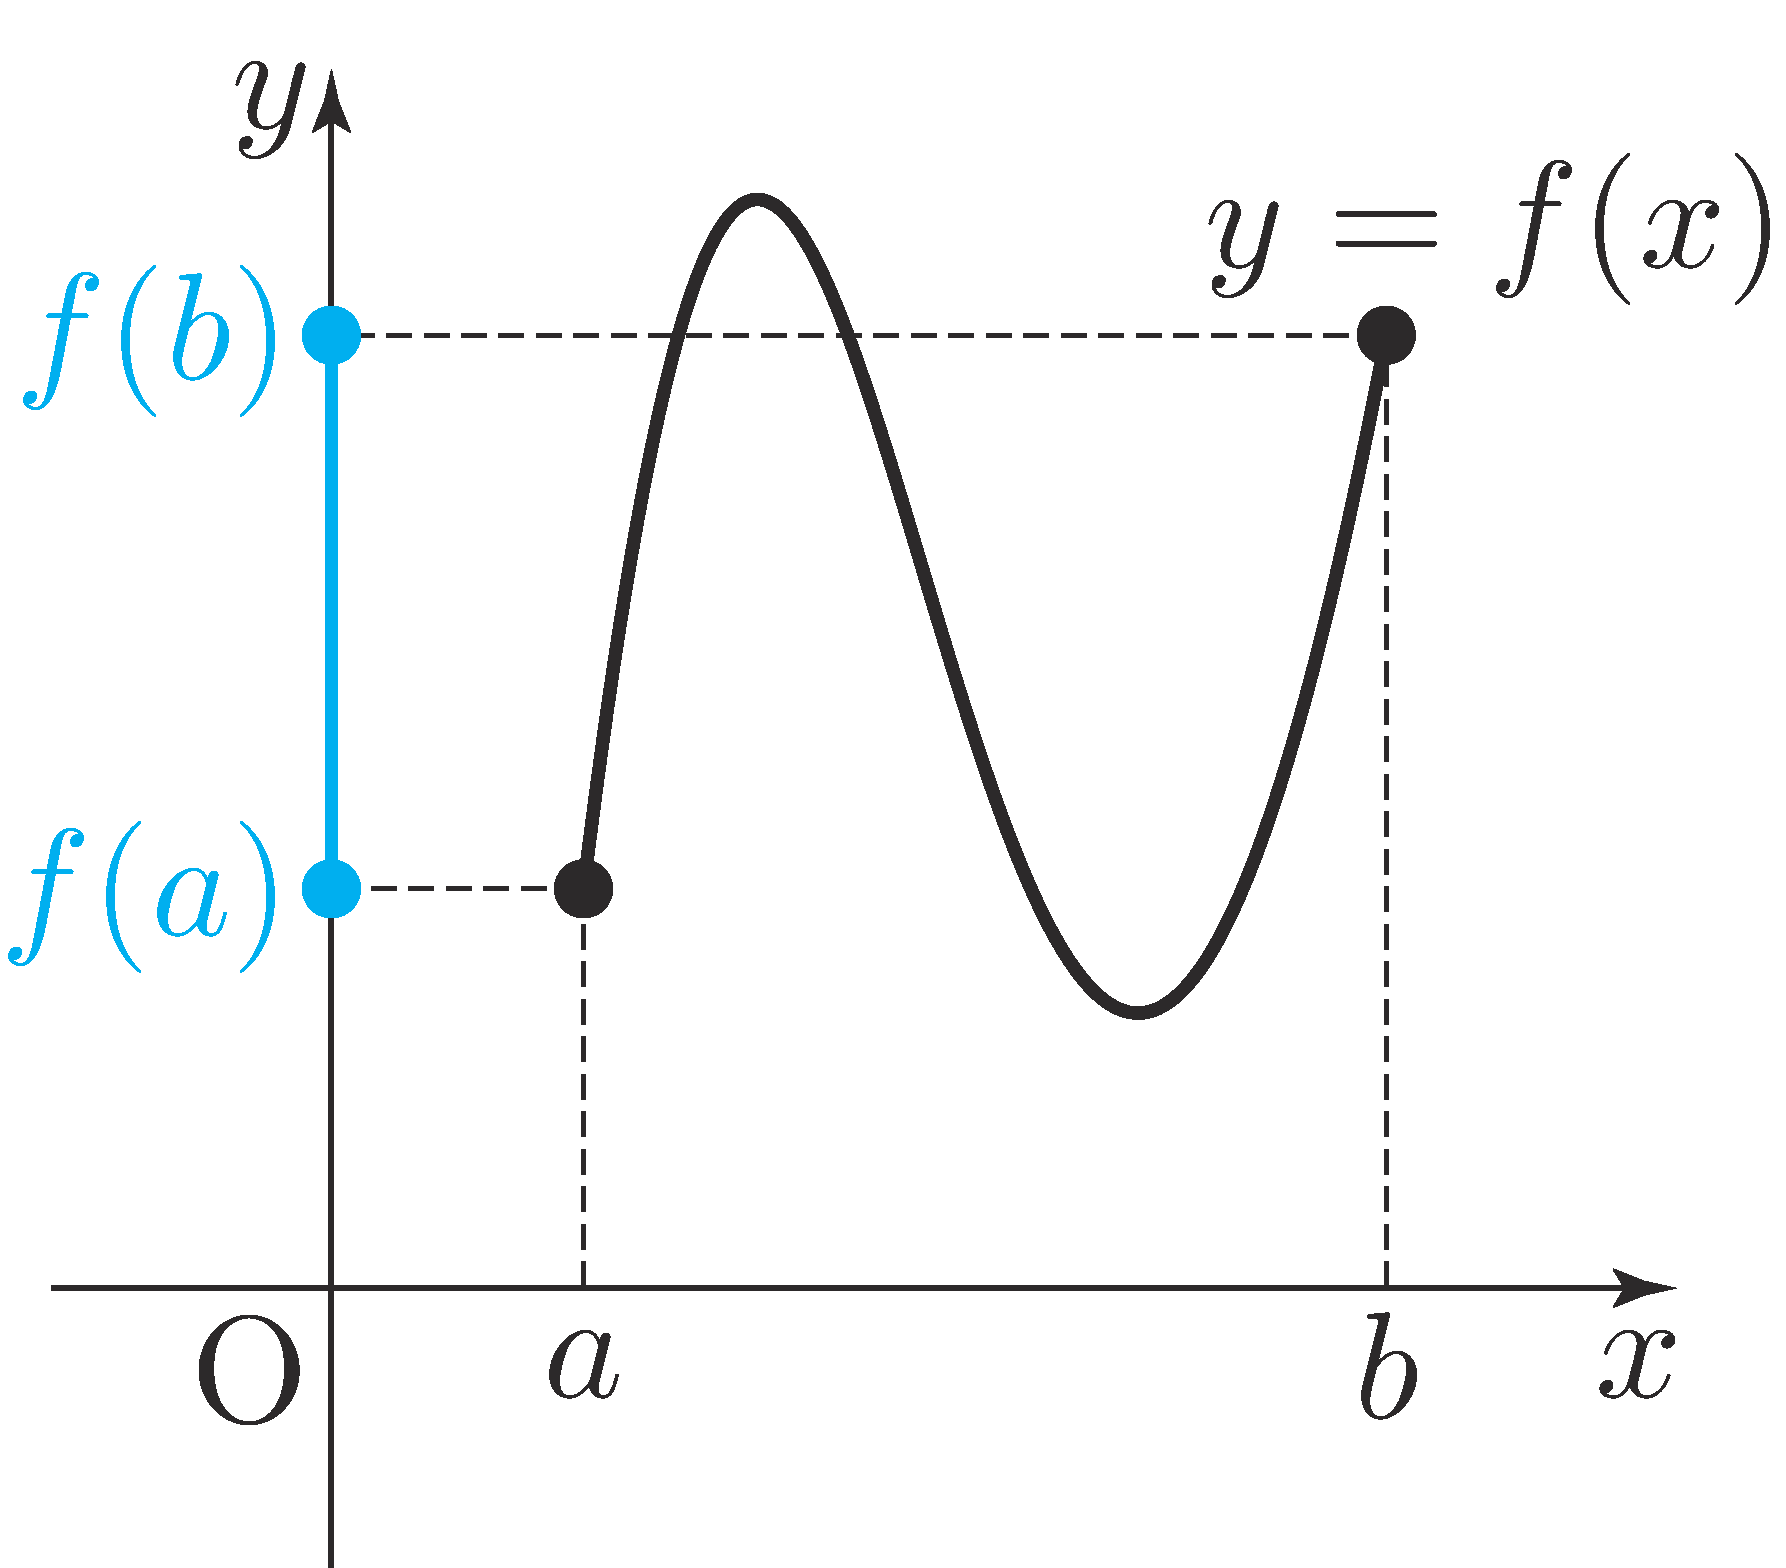
\includegraphics[scale=\pgfkeysvalueof{picsize}]{DBs/pic/zerg_07.pdf}\
	\end{center}사잇값 정리에 따르면, 닫힌구간 $\CCI{a}{b}$에서 연속인 함수 $f\left( x \right) $의 치역은 닫힌구간 $\CCI{f\left( a \right) }{f\left( b \right) }$에 포함된 모든 실수 $y$를 포함합니다. 즉 $y$가 부등식 $f\left( a \right) \le y \le f\left( b \right) $를 만족한다는 사실과 더불어 $\CCI{f\left( a \right) }{f\left( b \right) }$ 사이의 모든 실수 값을 \dotemph{빠짐없이} 가질 수 있음을 이야기하는 것입니다.\mn[-6\blskip]{본문과 같이 $f\left( a \right) <f\left( b \right) $일 때는 닫힌구간 $\CCI{f\left( a \right) }{f\left( b \right)}$와 부등식 $f\left( a \right)  \le y \le f\left( b \right) $를 생각합니다. 본문과 달리 $f\left( a \right) >f\left( b \right) $일 때에는 닫힌구간 $\CCI{f\left( b \right) }{f\left( a \right) }$와 부등식 $f\left( b \right)\le y \le f\left( a \right) $를 생각합니다.}{}
\clearpage
\subsection{\Mmi{} 정리와 사잇값 정리를 종합하기}
연속함수에 대한 두 정리를 엮어봅시다. 닫힌구간 $\CCI{a}{b}$에서 연속인 함수 $f\left( x \right) $가 최댓값을 갖도록 하는 $x$의 값을 $d$, 최솟값 $m$을 갖도록 하는 $x$의 값을 $e$라 하겠습니다.

닫힌구간 $\CCI{a}{b}$에서 $f\left( x \right) $의 치역은 닫힌구간 $\CCI{d}{e}$\mn{$d$와 $e$의 대소관계에 따라 $d<e$이면 $\CCI{d}{e}$, $d>e$이면 $\CCI{e}{d}$를 잡습니다.}{}에서의 $f\left( x \right) $의 치역을 포함합니다.
닫힌구간 $\CCI{d}{e}$에서는 $y$가 $\CCI{m}{M}$ 사이에 포함된 모든 실수의 값을 \dotemph{빠짐없이} 가질 수 있으며, 이 범위는 $f\left( x \right) $의 최솟값 $m$부터 최댓값 $M$까지 전부를 포함합니다.
\begin{center} 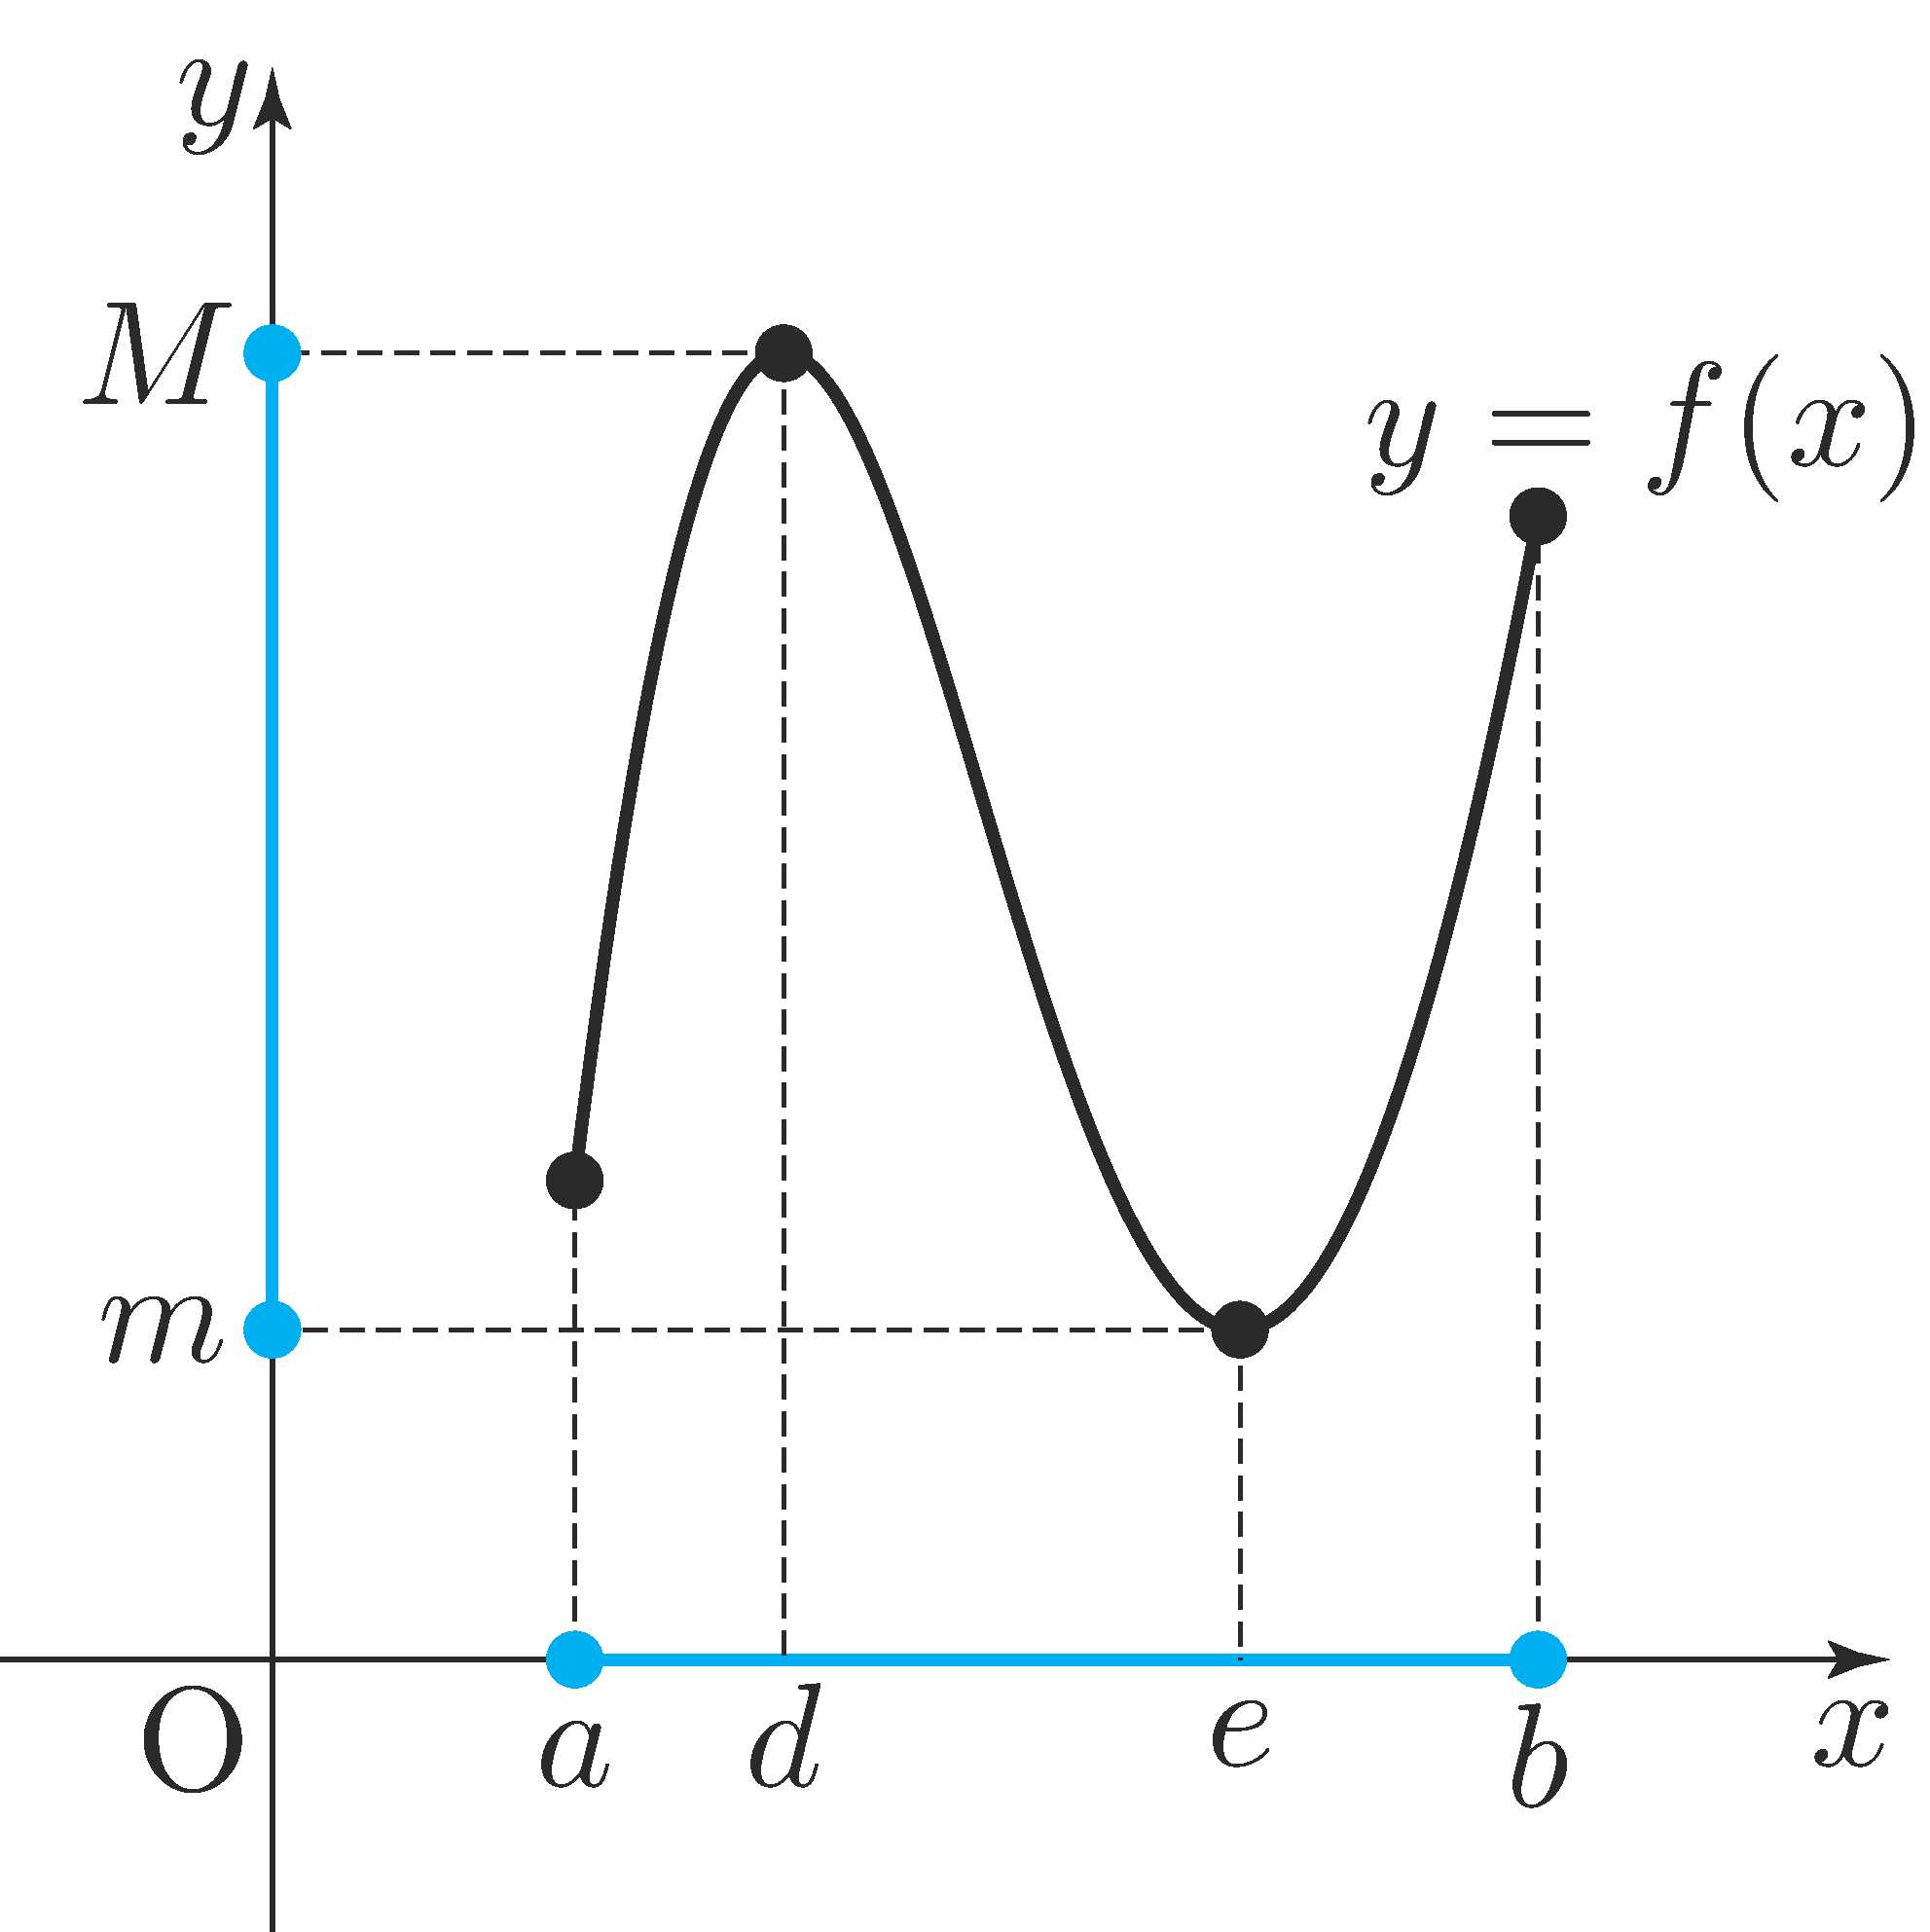
\includegraphics[scale=\pgfkeysvalueof{picsize}]{DBs/pic/zerg_08.pdf}\
	\end{center}따라서 닫힌구간 $\CCI{a}{b}$에서 $f\left( x \right) $의 치역은 닫힌구간 $\CCI{m}{M}$에 포함된 모든 실수 $y$입니다. 이를 말로 풀어보면 다음과 같이 해석할 수 있습니다.\begin{center}
    연속함수의 정의역이 닫힌구간 $\CCI{a}{b}$에서 끊어지지 않고 이어져 있으면\\
    연속함수의 치역은 닫힌구간 $\CCI{m}{M}$에서 끊어지지 않고 이어져 있다.
\end{center}